\documentclass{acm_proc_article-sp}

\usepackage{hyperref}

\begin{document}

\title{Thinking model and machine understanding of English primitive texts and it's application in Infrastructure as Service domain.}

\numberofauthors{3}
\author{
% 1st. author
\alignauthor Alexander Toschev\\
       \affaddr{Kazan State University}\\
       \affaddr{Universitetskaya 17,}\\
       \affaddr{420008 Kazan, Russia}
       \email{alexander.toschev@gmail.com}
% 2nd. author
\alignauthor Max Talanov\\
       \affaddr{Kazan State University}\\
       \affaddr{Universitetskaya 17,}\\
       \affaddr{420008 Kazan, Russia}
       \email{max.talanov@gmail.com}
% 3rd. author
\alignauthor Andrey Krekhov\\
       \affaddr{Fujitsu GDC Russia, Kazan}\\
       \affaddr{Sibirskii trakt 34,}\\
       \affaddr{420029 Kazan, Russia}
       \email{andrey.krekhov@ts.fujitsu.com}
}

\date{22 February 2013}

\maketitle

\begin{abstract}

Construction of machine understanding is definitely the challenge. There are several technologies used widely.
Currently mainstream applications uses machine operatable knowledge bases, for example \href{http://www.wolframalpha.com}{Wolfram Alpha} to support simple dialog and operate devices.
Newer the less those approaches do not create machine understanding of even primitive incidents.
We tried new approach based on assumption that human understanding is tightly coupled with human thinking itself.
We used thinking model described in Marvin Minsky book \href{http://en.wikipedia.org/wiki/The_Emotion_Machine}{"The emotion machine"}.

\keywords{AI, machine understanding, it outsourcing}

\end{abstract}

\section{The emotion machine thinking model}
\subsection{6 thinking levels}

\href{http://web.media.mit.edu/~minsky/E5/eb5.html}{Marvin Minsky} introduces the thinking as layered model that contains 6 layers:

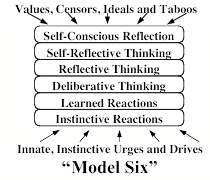
\includegraphics[scale=0.9]{model_6.png}

\begin{itemize}
 \item \emph{Instinctive Reactions}:  Joan hears a sound and turns her head. All animals are born equipped with ‘instincts’ that help them to survive.
 \item \emph{Learned Reactions}: She sees a quickly oncoming car. Joan had to learn that conditions like this demand specific ways to react.
 \item \emph{Deliberative Thinking}: To decide what to say at the meeting, she considers several alternatives, and tries to decide which would be best.
 \item \emph{Reflective Thinking}: Joan reflects upon what she has done. She reacts, not just to things in things in the world, but also to recent events in her brain.
 \item \emph{Self-Reflective Thinking}: Being "uneasy about arriving late" requires her to keep track of the plans that she's made for herself.
 \item \emph{Self-Conscious Thinking}: When asking what her friends think of her, she also asks how her actions concord with ideals she has set for herself.
\end{itemize}

Each upper layer controls lower layers, and is based on constructs and uses signals of lower layers as input.

\subsection{Selector, Critic, Way to think triple}

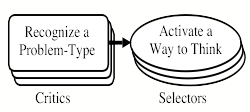
\includegraphics{critic_selector_model.png}


Marvin Minsky defines Critics - Selector behaviour as following:\\
On the left are resources that we shall call Critics, each of which can recognize a certain species of "Problem-Type". When a Critic sees enough evidence that you now are facing its type of problem, then that Critic will try to activate a "Way to Think" that may be useful in this situation.

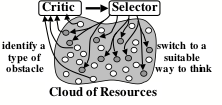
\includegraphics{critic_selector.png}

Critic -> Selector -> Way to think are main components that implements all the machine understanding process. Critics could be understood as probabilistic predicates that does analysis of current context in memory. Selector retrieves resources from memory. Way to think is main worker that updates current context in memory.

\section{Implementation of thinking model}

We have implemented thinking model described above over the infrastructure as service domain. Main unit of information to be processed is incident: the issue with description.

\subsection{Thinking levels control}

6 thinking levels are implemented by ThinkingLifeCycle component. It starts and controls and implements collaboration of actions: critics or ways to think that are assigned to different thinking layers. ThinkingLifeCycle also controls context of current incident processing in short term memory. It also controls goals orientation: to make whole machine understanding process oriented to the main goal: help user.\\

\begin{itemize}
  \item Critics are implemented as functions that returns selector request with probability and confidence.
  \item Selector runs requests and retrieves resources from memory(first from short term then from long term).
  \item Way to think are implemented as components that actually changes the contents of short term memory.
\end{itemize}

\subsection{Memory: short term, long term}

Memory is something that are associated with structures and objects in RAM and stored in Knowledge Base(KB) information.
There are two types of memory: Short term and Long term.

\subsubsection{Short term memory}

It stores the current context of incident processing. Eventually all objects from Short term memory should be stored in Long term memory. This is done via confirmation process and then machine learning (training). 
Training is based mainly on three mechanisms:
\begin{itemize}
  \item Deduction(Reasoning from generalised rules to specific)
  \item Induction(Generalisation)
  \item Abduction
\end{itemize}

\subsubsection{Long term memory}

Stores persistent information mainly in the KB, this information has following main structures:

\begin{itemize}
  \item Narrative
  \item Semantic network (mainly: Semantic network of concepts)
  \item Knowledge line: list of references, that addresses concepts in different domains.
\end{itemize}

\section{IS domain application of the thinking model}

Infrastructure as service domain contains 60 percent (according to our estimates) of incidents: issues that are mainly simple or primitive issues related to connectivity or software problems on a customer machine. 

\subsection{Critics and ways to think for incident processing}

All the mechanisms described above introduces main mechanisms of the thinking model. Simplified incident understanding process(only three layers) is described below.

\subsection{Preliminary processing}

First of all, on the Learned layer: textual description should be translated in to the form Semantic network this structure is stored in Short term memory, in following steps:

\begin{itemize}
  \item Preliminary splitting
  \item Knowledge base annotation
  \item Lexical parsing
\end{itemize}

Goal manager selects next goal: Classify incident.

\subsection{Incident classification}

On the Learned layer: three critics are invoked: 
\begin{itemize}
  \item Direct instruction analyser
  \item Problem description without desired state analyser
  \item Problem description with desired state analyser
\end{itemize}

All those critics returns probability of each case (selector request) that are processed by Get most probable action analyser. Most probable selector request is been processed immediately all the rest are stored in short term memory. Then goal manager select next goal: generate the solution.

\subsection{Direct instruction processing}

Solution search mechanism searches for the solution based on direct instruction semantic network, fist in short term memory then in long term memory.

\subsection{Problem description processing}

Problem description should be reformulated in form:
\begin{itemize}
  \item What's wrong
  \item Problem source
  \item Problem location references
\end{itemize}

Then solution search mechanism is started and returns solution with probability of match. If no proper solution found system rises Cry for help(way to think) and is reported to human operator.

\subsection{References}

\end{document}